\chapter{Introduction}
\label{chap:intro}
% add the sections
\section{Background of the Study}
A workflow consists of three dimensions, namely the process, resource, and case dimension \cite{hollingsworth}.  The process dimension is a specification of a process, the process being a partial ordering of a set of tasks such as control schemes like sequential, conditional, or iteration. The resource dimension pertains to the resource specification, where a resource is an object in the system that performs calculations, or processes, a task. Finally, the case dimension is the specification of the case, where case refers to the abstraction of a set of entities executed according to how the process is defined by the proper resource. \cite{Aalst1996} \cite{Malinao2017}.

\begin{figure}
    \centering
    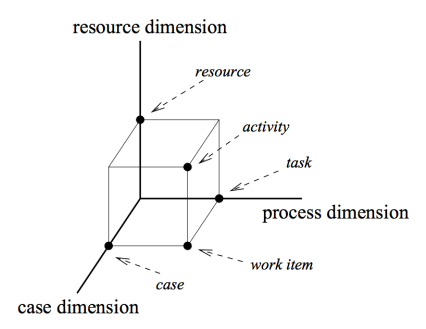
\includegraphics[width=8cm]{../figures/Workflow Dimensions.png}
    \caption{The three dimensions of workflows. (Image source:\cite{Malinao2017})}
    \label{WorkflowDimensions}
\end{figure}

Workflow models use complex and dynamic real-world systems in various fields such as human resource management,  biology (integrated disease surveillance [Lopez et al. 2020]),  and manufacturing engineering (chiller systems \cite{Ramirez2024}). This includes models such as Petri nets (PN) and Robustness Diagrams with Loop and Time Controls (RDLT) \cite{Malinao2017}. These models allow workflow components to be analyzed and model properties to be verified. \\

The study of the workflow model RDLT has been important in recent years due to its capability to represent a workflow in all of its dimensions (process, resource, and case). Although there are other workflow models that can represent all dimensions e.g. business process modeling and notation (BPMN), activity diagrams, etc., there are gaps and challenges in verifying the properties of these models. Issues like concept excess, lack of support for explicit representation of data and rules, functional decomposition, etc. This is partly due to the separation of the represenation of the resources in a workflow to the actual processes. RDLT solves such problems, for example, by using abstractions of encapsulated activities that can be controlled by external processes (e.g., Reset-Bound Systems). In short, RDLT provides mechanims that effectively intgerate all three workflow dimensions. \cite{Malinao2017} \\

Soundness in Workflow Nets, eventually refered to as classical soundness, refers to the property of a workflow to be absent of livelocks, deadlocks, and other anomalies in the flow \cite{Aalst1996}. In general, to be classically sound, a model should have proper termination and liveness. There are other variations of soundness focusing on specific relaxations or modifications of the conditions proper termination and liveness, namely, relaxed, weak, easy, and lazy soundness. In the context of RDLTs, being a relatively newer workflow model, current literature shows some formalizations on notions of soundness. Classical soundness in RDLT was defined in \cite{MalinaoPJS2023} as well as relaxed soundness. Weak and easy soundness was later defined and formalized as well in \cite{Ramirez2024}. Meanwhile, easy soundess in the context of RDLT is yet to be properly defined. \\ 

Hence, with all the knowledge about workflows and RDLT's notions of soundness, further research would expand in terms of automation to verify model properties. Therefore, various research has been done about the representation of RDLT into mathematical models aiming to automize verification. In Karen and Roben's work \cite{KarenRoben2018}, they proposed a matrix representation of RDLT to verify soundness. Asoy \cite{Asoy2024} used a matrix representation of RDLT to verify and automate classical soundness. This paper aims to leverage the structural and behavioral profile of weak and easy soundness as formally defined in \cite{Ramirez2024} and use matrix representations and operations to verify these notions of soundness in an RDLT. \\

The content of this paper is outlined as follows: Section \ref{sec: BasicDefNot} describes the basic definitions and notations of the current literature necessary to understand the topic at hand. Under this section describes brief background on Workflow Nets, Petri Nets, and its notions of soundness. It follows then the discussion on formal definitions of RDLT and its notions of soundness. Important algorithms in RDLT such as activity extraction (algorithm \ref{ActivityExtraction}) and vertex simplifications (algorithms \ref{vertexSimplification} \ref{EVSA}) are described as well, including the concepts and definitions necessary. Section \ref{sec:ProbStmnt} to \ref{sec:TCF} outlines this paper's problem statement, aim, scope and limitations, significance, and the theoretical and conceptual framework of the study, respectively. Chapter \ref{chap:RRL} describes the methodology and important findings of important literatures.

\section{Basic Definitions and Notations}
    \label{sec: BasicDefNot}
%  add subsections for petri nets and workflows
\subsection*{Petri Nets}
% description for petri net, what is it, what is its characteristics and why is important
Petri Net \cite{Petri1962} is a type of workflow model conceptualized by Carl Adam Petri in his disseration  \emph{Kommunikation mit Automaten} (Communication with Automata) in 1962. This model became the basis for most modelling framework, or was inspired thereof \cite{Malinao2017}. Although having to only represent a workflow of its case and process dimensions, understanding Petri Nets and its notions of soundness (as in Workflow Nets) can also aid in our understanding of the notions of soundness in RDLT, as it is what these prior notions of soundness were built upon. \\

A Petri Net is a bipartite graph composed of two types of nodes, namely, places (represented by a circle) and transitions (represented by a rectangle), and an arc, which connects nodes only of different types (place to transtion, and vice versa). \\
A place can either be an \emph{input}  or \emph{output} place. A place is said to be satisfied if there is at least one token inside of the place, and if it is satisfied (also called enabled), it may fire in which every output place it has recieves one token \cite{Petri1962}. \\ 

The following sections defines Petri Nets and Worklow Nets, which is a particular class of Petri Net, and follows the definitions of notions of soundness in Workflow Nets. These are important to understand as they are the basis for the formulization of the notions of soundness in the context of RDLT. The definitions in this section are mainly taken from papers \cite{Malinao2017} \cite{MalinaoPJS2023} \cite{Aalst2011} \cite{Aalst1996}with descriptions for supplemantary explanations.

% DEF: Petri Nets
\begin{defn}\textbf{Petri Nets and Markings} \cite{Aalst1996} \cite{MalinaoPJS2023}
    \label{PetriDef}
    A Petri Net is $ (P,T,F,M_0) $ which is a tuple that consists of four elements:
    \begin{itemize}
        \item a set of places $ P $ 
        \item a set of transition $ T $ where the intersection of places and transitions must not be empty
        \item a set of arcs $ F $ which is a subset of the union of all the possible connections from places to transitions and vice versa.
        \item an initial marking $ M_0 : P \rightarrow \mathbb{N}$
    \end{itemize}
\end{defn}

Figure \ref{PNComponents} shows the components of a Petri Net. 

\begin{figure}[H]
    \centering
    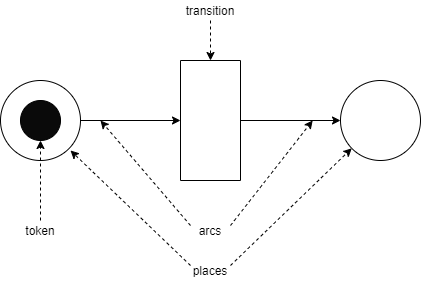
\includegraphics[width=10cm]{../figures/PN Components.png}
    \caption{The components of a Petri Net}
    \label{PNComponents}
\end{figure}

% TODO: (DONE) Add Illustration of Petri Nets
% TODO: Include definitions of Workflow Nets and its notions of Soundness
\subsection*{Soundness in Workflows}
A \emph{Workflow Net} (WF-Net) is a class of Petri Net that offer capabilities of the analysis of parallel execution of activities across splits and joins of processes \cite{Malinao2017}. 
% DEF: Strongly Connected
\begin{defn}\textbf{Strongly Connected} \cite{Malinao2017}\\
    \label{StrongConnDef}
    A Petri Net is \textbf{strongly connected} if there exists a path from $x$ to $y$ for every pair of nodes $x$ and $y$.
\end{defn}
% Description of Definition: Strongly Connected
Figure \ref{PNComponents} shows a simple Petri Net where every possible pair of nodes are connected, hence a \textbf{strongly connected} Petri Net. 

% DEF: Workflow Net
\begin{defn}\textbf{Workflow Nets} \cite{Malinao2017}\\
    \label{WNDef}
    A Petri Net is a \textbf{Workflow Net} if such a Petri Net holds the following conditions:
    \begin{itemize}
        \item The Petri Net contains two special places which are a source place $ i $ that does not have any input places and a sink place $ o $ that does not have any output places.
        \item The Petri Net is strongly connected if the source place $ i $ and the sink place $ o $ are connected to a transition $ t* $, as an input and output place respectively.
    \end{itemize}
\end{defn}
Given the two conditions outlined above, this would mean that the Petri Net in Figure \ref{PNComponents} is a Workflow Net.

% DEF: Workflow Nets (DONE)
On the literature of Workflow Nets, all notions of soundness are already established. The notions of soundness in the context of Workflow Nets are shown in a heirarchy in Figure \ref{SoundnessRelationships}, where arrows show a relationship of implication.

\begin{figure}[H]
    \centering
    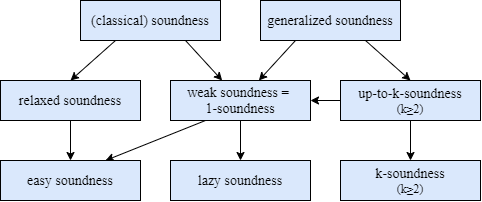
\includegraphics[width=13cm]{../figures/Relationships between Soundness Notions.png}
    \caption{Relationships between the different soundness notions where the arrows represent the implication of relationships from one notion to another. (Image source: \cite{Aalst2011})}
    \label{SoundnessRelationships}
\end{figure}
In the next sections, only classical soundness, relaxed soundness, weak, and easy soundness are discussed, as they are the ones relevant to understanding weak and easy soundness in the context of RDLT, to be discussed in further sections.

% DEF: Classical Soundness of Workflow Nets
\begin{defn}\textbf{Classical Soundness of Workflow Nets} \cite{Aalst2011}\\
    \label{ClassicalWNDef}
    A Workflow Net is classical sound if and only if the following requirements are satisfied:
    \begin{itemize}
        \item Option to complete: the sink place $ o $ is reachable from the source place $ i $.
        \item Proper termination: the sink place $ o $ receives exactly one token and all other places must be empty.
        \item Liveness: every transition must be involved in at least one process specification.
    \end{itemize}
\end{defn}
This notion of soundness offeres a very strict criterion since it imposes that all process for each case are complete, leaving no pending, or cancelled task when the token reaches the sink, as explained in condition 2. \cite{Malinao2017} Figure \ref{PNComponents} shows a classically sound workflow net.
Sytems also allow the implementation of a workflow wherein at least every transition is involved in a case that is properly completed, or a token reaches the sink. This variation of soundness is less restrictive compared to that of a classically sound workflow net. The criterion is weakened to some degree, hence the following notions of soundness:
% DEF: Relaxed Soundness of Workflow Nets
\begin{defn}\textbf{Relaxed Soundness of Workflow Nets} \cite{Aalst2011}\\
    \label{RelaxedWNDef}
    A Workflow Net is of relaxed sound if and only if the following requirements are satisfied:
    \begin{itemize}
        \item Option to complete: the sink place $ o $ is reachable from the source place $ i $.
        \item Proper termination (weakened): at least one case exists that completes with one token in the sink place $ o $ with other places being empty.
        \item Liveness: every transition must be involved in at least one process specification.
    \end{itemize}
\end{defn}

In relaxed soundness, the proper termination is weakened to at least one case in the workflow net exist where it completes with one token in the sink $o$ while other places are empty. Therefore, it allows other cases where the workflow terminates while still having processes working in the background, represented in the model by a token inside a place, as shown in Figure \ref{WNRelaxed}. Similarly, since classical soundness is implied in a relaxed sound workflow net, Figure \ref{PNComponents} is also of relaxed sound.

\begin{figure}[H]
    \centering
    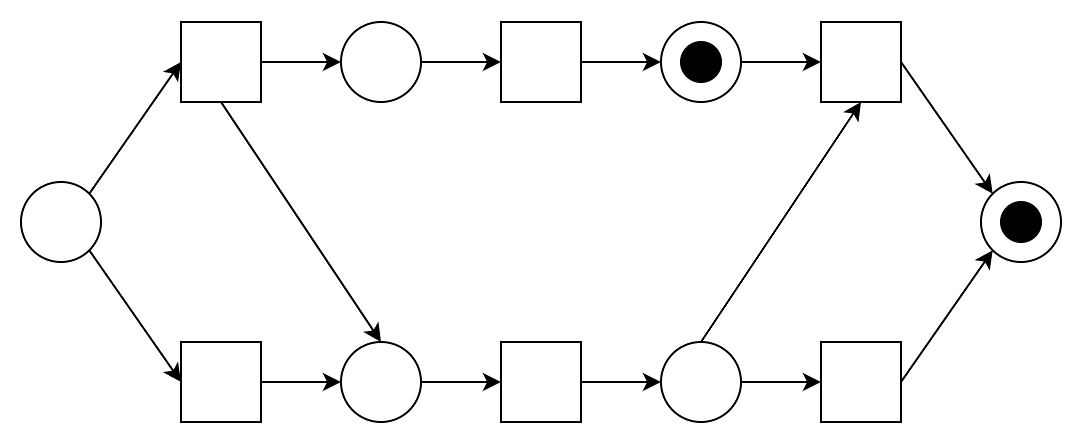
\includegraphics[width=11cm]{../figures/RelaxedSoundWFNet.png}
    \caption{A Workflow Net of Relaxed Soundness (Adopted From: \cite{Aalst2011})}
    \label{WNRelaxed}
\end{figure}
% DEF: Weak Soundness of Workflow Nets
\begin{defn}\textbf{Weak Soundness of Workflow Nets} \cite{Malinao2017}\\
    \label{WeakWNDef}
    A Workflow Net is of weak sound if and only if the following requirements are satisfied:
    \begin{itemize}
        \item Option to complete: the sink place $ o $ is reachable from the source place $ i $.
        \item Proper termination: the sink place $ o $ receives exactly one token and all other places must be empty.
    \end{itemize}
\end{defn}
On weak soundness in workflow nets, only two conditions are required, as defined above. The workflow should have an option to complete, and it should properly terminate. In comparison to classical soundness, it does not require liveness, that is every transition be live for every execution. An example of a weak sound workflow net is found in Figure \ref{WeakSoundWFNet}. This net is not classically sound since $t_3$ is a dead transition, making the workflow net not live and not fulfilling the third condition of a classically sound workflow net. 

\begin{figure}[H]
    \centering
    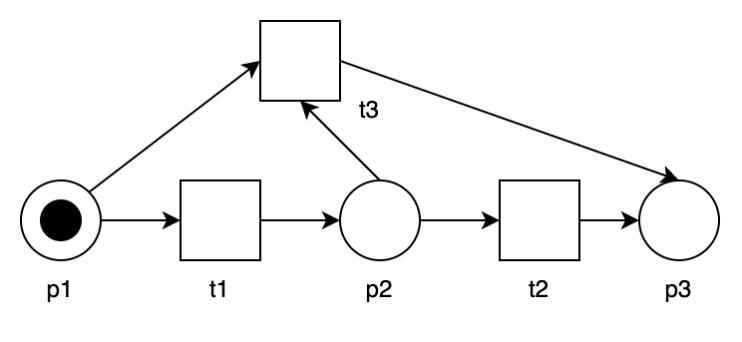
\includegraphics[width=8cm]{../figures/WeakSoundWFNet.png}
    \caption{A Workflow Net of Weak Soundness (Adopted from: \cite{Aalst2011})}
    \label{WeakSoundWFNet}
\end{figure}

% DEF: Easy Soundness of Workflow Nets
\begin{defn}\textbf{Easy Soundness of Workflow Nets} \cite{Malinao2017}\\
    \label{EasyWNDef}
    A Workflow Net is of easy sound if and only if the following requirement is satisfied:
    \begin{itemize}
        \item Option to complete: the sink place $ o $ is reachable from the source place $ i $.
    \end{itemize}
\end{defn}
Easy soundness in the context of workflow nets only has one condition as defined above, that is it should have an option to complete. Similarly, in Figure \ref{WNEasy}, transition $t_1$ to $t_2$ leads to the sink $o$, hence has an option to complete. However, it does not satisfy the other conditions of other notions of soundness.

\begin{figure}[H]
    \centering
    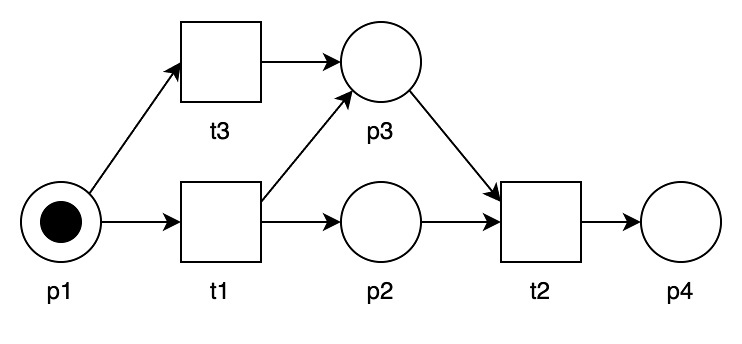
\includegraphics[width=8cm]{../figures/EasySoundWFNet.png}
    \caption{A Workflow Net of Easy Soundness (Image source: \cite{Aalst2011})}
    \label{WNEasy}
\end{figure}
% TODO: Add the figure of the soundness in workflow nets

As a summary and ease of reference, the table below maps the requirements of soundness in the context of workflow nets \ref{SoundnessReqs}, obtained from \cite{Ramirez2024}.
%  definition of Workflow Nets 
% \begin{table}[H]
%     \centering
%     \caption{Requirements of the Soundness Notions of Workflow Nets} \cite{Ramirez2024}
%     \label{SoundnessReqs}
%     \begin{tabular}{|l|*{5}{c|}}
%         \hline
%         \backslashbox{Requirement}{Soundness Notion} & Classical & Relaxed & Weak & Lazy & Easy \\
%         \hline
%         Option to complete & \cellcolor{LightBlue} & \cellcolor{LightBlue} & \cellcolor{LightBlue} & \cellcolor{LightBlue} & \cellcolor{LightBlue} \\
%         \hline
%         Proper termination & \cellcolor{LightBlue} &  & \cellcolor{LightBlue} &  &  \\
%         \hline
%         Proper termination (weakened) &  & \cellcolor{LightBlue} &  & \cellcolor{LightBlue} &  \\
%         \hline
%         Liveness & \cellcolor{LightBlue} & \cellcolor{LightBlue} &  &  &  \\
%         \hline
%     \end{tabular}
% \end{table}
% \
% \begin{table}[H]
%     \centering
%     \caption{Requirements of the Soundness Notions of Workflow Nets \cite{Ramirez2024}}
%     \label{SoundnessReqs}
%     \begin{tabular}{|l|*{5}{c|}}
%         \hline
%         \diagbox{Requirement}{Soundness} & Classical & Relaxed & Weak & Lazy & Easy \\
%         \hline
%         Option to complete & \cellcolor{LightBlue} & \cellcolor{LightBlue} & \cellcolor{LightBlue} & \cellcolor{LightBlue} & \cellcolor{LightBlue} \\
%         \hline
%         Proper termination & \cellcolor{LightBlue} &  & \cellcolor{LightBlue} &  &  \\
%         \hline
%         Proper termination (weakened) &  & \cellcolor{LightBlue} &  & \cellcolor{LightBlue} &  \\
%         \hline
%         Liveness & \cellcolor{LightBlue} & \cellcolor{LightBlue} &  &  &  \\
%         \hline
%     \end{tabular}
% \end{table}

% -------------------------------------------
\subsection*{Robustness Diagram with Loop and Time Controls}
In this section, RDLT and its notions of soundness are defined. RLDT is a workflow model that allows all three dimension of a workflow to be represented.

\begin{defn}\textbf{RDLT} \cite{Malinao2017}\\
    \label{RDLTDef}
    An RDLT is a graph representation \begin{math}R\end{math} of a system that is defined as \begin{math}R = (V, E, T, M)\end{math} where:
    \begin{itemize}
        \item \begin{math}V\end{math} is a finite set of vertices, where each vertex has a type \begin{math}V_{type}: V \rightarrow \end{math} \{'b', 'e', 'c'\} where 'b', 'e', and 'c' means the vertex is either a "boundary object", an "entity object", or a "controller", respectively.
        
        \item A finite set of arcs \begin{math}E \subseteq (V \times V) \backslash  E'\end{math} where \begin{math}E' = \{(x,y) | x,y \in V, V_{type}(x) \in \end{math} \{'b', 'e'\}, \begin{math}V_{type}(y) \in \end{math} \{'b', 'e'\}\} with the following attributes with user-defined values,
            
            \begin{itemize}
                \item \begin{math}C : E \rightarrow \Sigma \cup \{\epsilon\} \end{math} where $\Sigma$ is a finite non-empty set of symbols and $\epsilon$ is the empty string. Note that for real-world systems, a task \begin{math}v \in V\end{math}, i.e. \begin{math}V_{type}(v) = \end{math}'c', is executed by a component \begin{math}u \in V, V_{type}(u) \in \end{math} \{'b','e'\}. This component-task association is represented by the arc \begin{math}(u, v) \in E \end{math} where \begin{math}C((u,v)) = \epsilon\end{math}. Furthermore, \begin{math}C((x,y)) \in \Sigma\end{math} represents a constraint to be satisfied to reach \begin{math}y\end{math} from \begin{math}x\end{math}. This constraint can represent either an input requirement or a parameter \begin{math}C((x,y))\end{math} which needs to be satisfied to proceed from using the component/task \begin{math}x\end{math} to \begin{math}y\end{math}. \begin{math}C((x,y)) = \epsilon\end{math} represents a constraint-free process flow to reach \begin{math}y\end{math} from \begin{math}x\end{math} or a self-loop when \begin{math}x = y\end{math}.
                
                \item \begin{math}L : E \rightarrow \mathbb{Z}\end{math} is the maximum number of traversals allowed on the arc.
            \end{itemize}
        
        \item Let \begin{math}T\end{math} be a mapping such that \begin{math}T((x, y)) = (t1,...,tn)\end{math} for every \begin{math}(x, y) \in E\end{math} where \begin{math}n = L((x, y))\end{math} and \begin{math} t_{i} \in \mathbb{N}\end{math} is the time a check or traversal is done on \begin{math}(x, y)\end{math} by some algorithm’s walk on \begin{math}R\end{math}.
            
        \item \begin{math}M : V \rightarrow \{0,1\}\end{math} indicates whether \begin{math}u \in V\end{math} and every \begin{math}v \in V\end{math} where \begin{math}(u,v) \in E\end{math} and \begin{math}C((u,v)) = \epsilon\end{math} induce a sub-graph \begin{math}G_{u}\end{math} of \begin{math}R\end{math} known as a \textbf{reset-bound subsystem} (RBS). The RBS \begin{math}G_{u}\end{math} is induced with the said vertices when \begin{math}M(u) = 1\end{math}. In this case, \begin{math}u\end{math} is referred to as the \textbf{center} of the RBS \begin{math}G_{u}\end{math}. \begin{math}G_{u}\end{math}'s vertex set \begin{math}V_{G_{u}}\end{math} contains \begin{math}u\end{math} and every such \begin{math}v\end{math}, and its arc set \begin{math}E_{G_{u}}\end{math} has \begin{math}(x,y) \in E\end{math} if \begin{math}x,y \in V_{G_{u}}\end{math}.\\
        
        Finally, \begin{math}(a,b) \in E\end{math} is called an \textbf{in-bridge} of \begin{math}b\end{math} if \begin{math}a \notin V_{G_{u}}, b \in V_{G_{u}}\end{math}. Meanwhile, \begin{math}(b,a) \in E\end{math} is called an \textbf{out-bridge} of \begin{math}b\end{math} if \begin{math}b \in V_{G_{u}}\end{math} and \begin{math}a \notin V_{G_{u}}\end{math}. Arcs \begin{math}(a,b), (c,d) \in E\end{math} are \textbf{type-alike} if \begin{math}\exists y \in V\end{math} where \begin{math}(a,b), (c,d) \in Bridges(y)\end{math} with \begin{math}Bridges(y) = \{(r,s) \in E|(r,s)\end{math} is either an in-bridge or out-bridge of \begin{math}y\}\end{math} or if \begin{math}\forall y \in V, (a,b), (c,d) \notin Bridges(y)\end{math}.
    \end{itemize} 
\end{defn}

Figure \ref{sampleRDLT} shows an RLDT with a reset-bound system with center $x_2$ and its owned controllers $x_3$ and $x_4$. The in-bridges of the RBS with respect to $x_2$ are $(x_1, x_2)$ and $(x_6,x_2)$. Both arcs are type-alike with respect to $x_2$ as defined in \ref{RDLTDef}. However, $(x_3,x_2)$, being inside the RBS, is not type-alike to any of the aforementioned arcs. $(x_4, x_5)$ and $(x_4, x_6)$ are type-alike with respect to $x_4$.
For each arcs of this RDLT, $C-$ and $L-$ attributes are defined. The $x_1$ serves as the source, while the $x_7$ serves as the sink. 
\begin{figure} [H]
    \centering
    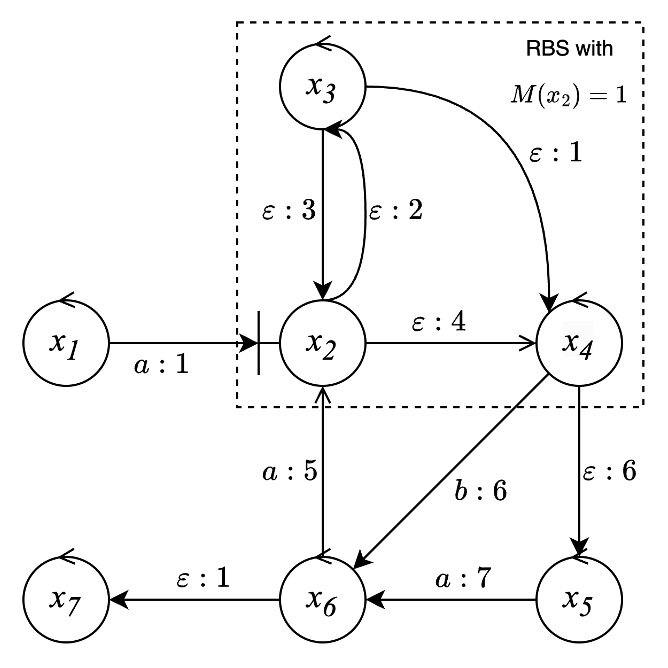
\includegraphics[]{../figures/sampleRDLTmain.png}
    \caption{A Reset-Bound Subsystem-Containing Robustness Diagram with Loop and Time Controls with center at $x_2$, where $M(x_2)=1$. (Adopted from: \cite{MalinaoWCTP2023})}
    \label{sampleRDLT}
\end{figure}
% Example RDLT (First Example)
% Figure \ref{RDLTComponents} shows an example of an RDLT based on the given definitions of the elements and the attributes that are labeled respectively. This RDLT also contains an RBS with the entity object $x2$ as the center of such RBS which is determined by its $M$-Attribute being equal to 1.\\
% \begin{Figure}[H]
%     \centering
%     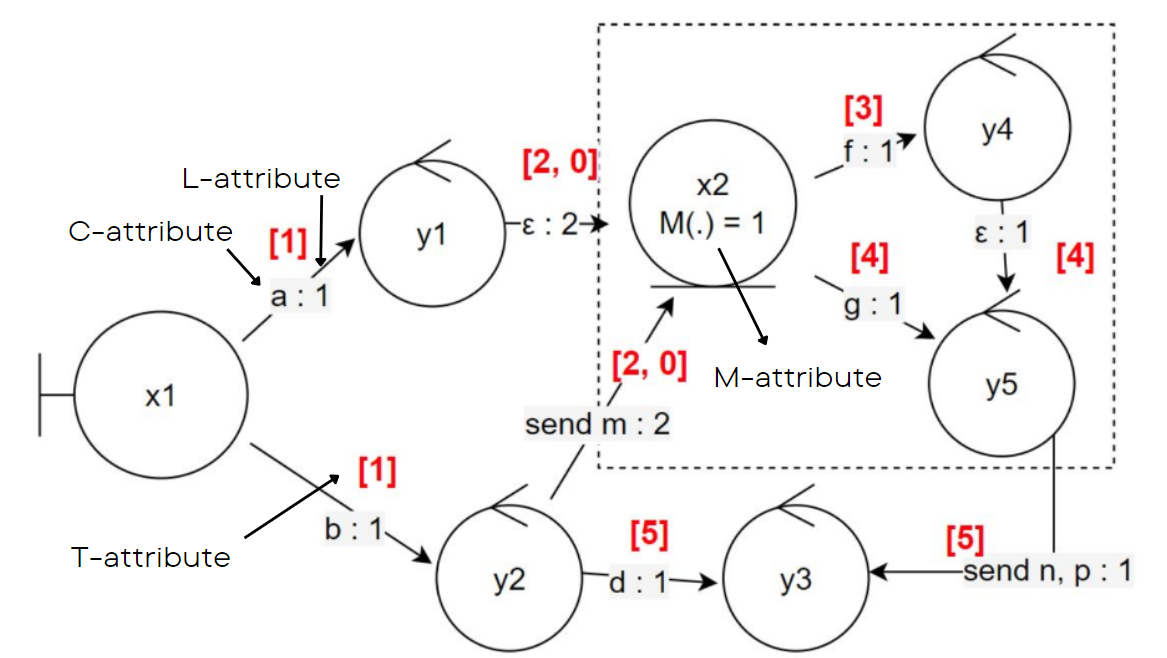
\includegraphics[width=12cm]{../Figures/RDLT Components.png}
%     \caption{A Labeled Reset-Bound Subsystem-Containing Robustness Diagram with a Boundary Object $x1$, an Entity Object $x2$, and Controllers $y1$, $y2$, $y3$, $y4$, and $y5$. (Image source: \cite{Sulla2023})}
%     \label{RDLTComponents}
% \end{Figure}

% -------------------------------------------
\subsection*{Activity Extraction Algorithm}
The proposed Algorithm \ref{ActivityExtraction} in paper \cite{Malinao2017}, called \emph{Activity Extraction Algorithm}, takes an input RDLT \emph{R} with a defined start index \emph{s} and goal vertex \emph{f}. As shown in Algorithm \ref{ActivityExtraction} it returns an \emph{activity profile} defined in Definition \ref{activityProfile}, a set of exected vertices from the extracted activities. To understand Algorithm \ref{ActivityExtraction} fully, along with the definition of \textbf{activity profile}, \textbf{reachability configuration}, defined in  Definition \ref{reachabilityConfiguration}, is introduced. Algorithm \ref{ActivityExtraction} is found at the appendices of this paper. 

% TODO: Include the description of activity extraction algorithm
%  ----
% DESCRIPTION OF ACTIVITY EXTRACTION
To perform \textbf{activity extraction} from vertex $x$, where $x = s$ at the start of algorithm \ref{ActivityExtraction}, the algorithm performs a \textbf{check}, defined in Algorithm \ref{alg:Check} in the appendices, on $x$ and other vertex $w \in E$  where $(x,w) \in E$. A \textbf{check}, defined in algorithm \ref{alg:Check} at the appendices, is a subroutine in $\mathcal A$ where $(x,y) \in E$ is arbitrarily selected, given that the number of traversals done on $(x,y)$ has not yet reached $L((x,y))$, which is the traversal limit of the arc, if such $y$ exists in $V$. Similarly, the constraint $C((x,y))$ is checked as well, and given both $L((x,y))$ and $C((x,y))$ are satisfied, then the arc $(x,y)$ is traversed and the next vertex in the workflow will be $y$. If this valid vertex $y$ is reached, the $\mathcal A$ assigns time step traversal value $t_i$. If a previous arc or an incoming arc $(u,x)$ prior to $(x,y)$, the time step $t_i$ is set to the maximum time step from all the time traversals $T((u,x))$ plus $1$ from the all the incoming arcs before $(x,y)$. Otherwise, the time traversal value is set to $1$, indicating the first traversal of the arc. 
After the check, $\mathcal A$ evaluates whether every $(v,y) \in E$, $v \in V$, does not prevent the traversal on $(x,y)$. When there are no constraints to the traversal on $(x,y)$, the said arc is said to be an \textbf{unconstrained arc}, as defined in \ref{unconstrainedarc}. On the other hand, if $(x,y)$ and $(v,y)$ are not type-alike, $(x,y)$ will not prevent traversal of $(x,y)$, and $(x,y)$ remains unconstrained with respect to all type-alike arcs with respect to the vertex $y$.

The following are the formal definitions of the concepts mentioned.
% ----

\begin{defn}\label{reachabilityConfiguration} 
    \textbf{Reachability Configuration} \cite{Malinao2017} \\
    A \textbf{reachability configuration} $S(t)$ in $R = (V, E, \Sigma, C, L, M)$ contains the arcs traversed by ${\mathcal A}$ at time step $t \in {\mathbb{N}}$.
\end{defn}

% ---- INCLUDE THE ALGORITHM FOR CHECK


\begin{defn}\label{activityProfile}
    \textbf{Activity Profile} \cite{Malinao2017} \\
    A set $S = \{S(1), S(2), \ldots,$ $S(d)\}$ of reachability configurations, $d \in {\mathbb{N}}$, is an \textbf{activity profile} in $R = (V, E, \Sigma, C, L, M)$ where $\exists(u,v) \in S(1)$ and $(x,y) \in S(d)$ such that $\nexists w, z \in V$ where $(w,u), (y, z) \in E$. 
\end{defn}
Essentially, a \textbf{reachability configuration} is the set of arcs traversed by activity extraction at a given time step $t_i$, while the \textbf{activity profile} of an RDLT is the set of all reachability configurations from time step $t_0$ to $t_d$, where $d$ is the step the workflow reached the sink. \\

Given these definitions, and following ${\mathcal{A}}$, the RDLT in Figure \ref{sampleRDLT} will have the following \textbf{reachability configuration}:
\begin{align*}
    S(1) &= \{(x_1, x_2)\}, \\
    S(2) &= \{(x_2, x_4)\}, \\
    S(3) &= \{(x_4, x_6), (x_4, x_5), (x_5, x_6)\}, \\
    S(4) &= \{(x_6, x_2)\}.
\end{align*}
The \textbf{activity profile} therefore of Figure \ref{sampleRDLT} is $S = \{S(1), S(2), S(3)\}$.

In step 4.3 of algorithm ${\mathcal{A}}$, an evaluation is performed to determine if $(x,y) \epsilon E$ is an unconstrained arc. The definition of an unconstrained arc is defined as follows:
\begin{defn} \label{unconstrainedarc}
    \textbf{Unconstrained Arc} \cite{Malinao2017} \\
    An arc $(x, y) \in E$ is \textbf{unconstrained} if $\forall (v,y) \in E$, where $(x,y)$ and $(v,y)$ are type-alike, any of the following traversal conditions hold, 
    \begin{enumerate}
        \item $C((v,y)) \in \{\epsilon, C((x,y))\}$,
        \item { $|\{t_i \in T((x,y))|t_i \geq 1\}| \leq  |\{t_j \in T((v,y))|t_j \geq 1\}|$ $\leq L((v,y)),$}
        \item $C((v,y)) \in \Sigma, C((x,y)) = \epsilon \wedge T(v,y) \neq [0]$.
    \end{enumerate}
    Note that $(x,y)$ will remain unconstrained (if it is such) regardless of any other $(v,y)$ where $(x,y)$ and $(v,y)$ are not type-alike.
\end{defn}

% -------------------------------------------

\subsection*{Vertex Simplification}
In RDLTs, subsystems of a workflow cause an increase in the complexity of its analysis. \textbf{Vertex simplification} aims to reduce this complexity through abstraction of the components of these subsystems. In this context, the RBS is subsystem being simplified in the process of vertex simplification, thus streamlining the structure of the diagram without losing essential information necessary for analysis.
\begin{defn}\textbf{Vertex Simplified $R$} \cite{Malinao2017}\\
    \label{VertexSimpDef}
     A vertex-simplified RDLT $ G $ = ($ V' $, $ E' $, $ C' $) of $ R = (V, E, T, M) $ (with arc attributes $ C $ and $ L $) is a multigraph whose vertices $ v \in $ V have $ V_{type}(v) = 'c' $ where $ G $ is derived from $ R $ such that the following holds:
     \begin{enumerate}
         \item $ x \in V' $ if any of the following holds:
         \begin{itemize}
             \item $ x \in V $ and $ x \notin V_{G_u} $ of an RBS $ G_u $ in $ R $, or
             \item there exists an in-bridge $ (q, x) \in E $ of $ x \in V \cap V_{G_u}, q \in V $ of $ R $, or
             \item there exists an out-bridge $ (x, q) \in E $ of $ x \in V \cap V_{G_u}, q \in V $ of $ R $, or
         \end{itemize}
         \item $ (x, y) \in E' $ with $ C'((x, y)) = C((x, y)) $ for $ x, y \in V' $ if $ (x, y) \in E $
         \item $ C((x, y)) = \varepsilon $ if $ x, y \in V' \cap V_{G_u} $ and $ x $ is an ancestor of $ y $ in $ R $ and $ (x, y) \notin E_{G_u} $  
     \end{enumerate}

     We refer to this simplification of $ R $ as \textbf{level-1 vertex simplification} of $ R $ with respect to every RBS $ G_u $ in $ R $. A \textbf{level-2 vertex simplification} of $ R $ with respect to its RBS $ G_u $ is the level-1 vertex-simplification of $ G_u $ where $ G_u $ is treated as an RDLT where the value of the vertex attribute $ M $ of $ u $ is redefined to $ 0 $, i.e. $ M(u) $ $ = $ $ 0 $. With this, the verification of model properties (i.e. maximally composed and sound RDLTs) are separately done for the level-1 and level-2 vertex simplifications of $ R $. However, this separation does not affect the validity of proving for any of these properties on the entire RDLT itself. 
 \end{defn}

Figure \ref{vertexSimplification} shows the vertex simplified form of the sample RDLT in Figure \ref{sampleRDLT}.

 \begin{defn}\textbf{Contraction of Arcs in RDLTs} \cite{Malinao2017}\\
    Given an RDLT $ R $ $ = $ $ (V,E,T,M) $ and its vertex-simplified RDLT $ G $ = $ (V',E',C') $, a contraction of $ (x,y) $ $ \in $ $ E' $ of $ G $, $ x $, $ y $ $\in $ $ V' $, $ x $ $ \neq $ $ y $, results to a multidigraph $ G* $ $ = $ $ (V*,E*,C*) $ such that:
    \begin{enumerate}
        \item $ V* $ $ = $ $ V'\backslash\{x,y\} \cup \{x'\} $. Here, $ x' $ is a dummy vertex representing $ x $ and $ y $.
        \item $ E* $ $ = $ $ \Bigl\{ E' \bigcup\limits_{\forall z \in V', \exists (z,v)_i \in E', v \in \{x,y\} } \bigl\{ \bigcup\limits_{\forall i} \bigl\{ (z,x')_i \bigr\} \bigr\} \bigcup\limits_{\forall z \in V', \exists (v,z)_j \in E', v \in \{x,y\} } \bigl\{ \bigcup\limits_{\forall j} \bigl\{ (x',z)_j \bigr\} \bigr\} \Bigr\} \backslash \\ \Bigl\{ \bigcup\limits_{\forall q \in V', \exists (q,v)_i \in E', v \in \{x,y\} } \bigl\{ \bigcup\limits_{\forall i} \bigl\{ (q,v)_i \bigr\} \bigr\} \bigcup\limits_{\forall q \in V', \exists (v,q)_j \in E', v \in \{x,y\} } \bigl\{ \bigcup\limits_{\forall j} \bigl\{ (v,q)_j \bigr\} \bigr\} \Bigr\}$, \\
        where $ z $ $ \notin $ $ \{x,y\} $, $ (a,b)_i $ $ \in $ $ E' $ is the $ i^{th} $ arc from $ a $ $ \in $ $ V' $ to $ b $ $ \in $ $ V' $, $ i $ $ = $ $ 1, 2, \ldots, n $, where $ n $ is the outdegree of $ a $.
        \item  $ C*((z,x')_i) $ $ = $ $ \varepsilon $, $ \forall z $ $ \in $ $ V' $ where $ \exists (z,y)_i $ $ \in $ $ E' $, $ i $ $ \geq $ $ 1 $,
        \item $ C*((x',z)_i) $ $ = $ $ C'((v,z)_i) $, $ v $ $ \in $ $ \{x,y\} $, $ \forall z $ $ \in $ $ V' $ where $ (v,z)_i $ $ \in $ $ E' $. $ i $ $ \geq $ $ 1 $.
    \end{enumerate}
\end{defn}
\textbf{Contraction of arcs in RDLT} involves the merging of two vertices into one \emph{dummy} vertex while still preserving the properties of the arcs involved. This allows the simplification of the RDLT by reducing the amount of vertices to be analyzed.

\begin{defn}\textbf{Feasible Contraction} \cite{Malinao2017}\\
    A contraction of $ (x,y) $ is feasible if $ \nexists (u,x) $ $ \in $ $ E' $ where $ C((u,x)) $ $ \in $ $ \Sigma $, $ u $ $ \in $ $ V' $ and\\
    \begin{gather*}
        \bigcup\limits_{\forall i}\{ C'((x,y)_i) \} \cup \{\varepsilon\} \supseteq \bigcup\limits_{\forall z \in V', \text{ where } \exists(z,y)_j \in E', j \geq 1 } \{ \bigcup\limits_{\forall i}\{ C'((z,y)_j) \} \},\\
    \end{gather*}
    where $ (x,y)_i $ $ \in $ $ E' $ is the $ i^{th} $ arc from $ x $ to $ y $, $ i $ $ = $ $ 1, \ldots, n $, and $ n $ is the outdegree of $ x $.
\end{defn}

By this definition, the validity of contraction of vertices $x$ and $y$ is evaluated. It is ensured in this condition that these vertices are correct hence can be contracted into a single vertex without violating any constraints of the arcs. This ensures unerroneaous behavior with the simplified RDLT.

\begin{defn}\textbf{Contraction Path in RDLTs} \cite{Malinao2017}\\
    \label{contractionPath}
    Given an RDLT $ R $ $ = $ $ (V,E,T,M) $ and its vertex-simplified RDLT $ G_1 $ = $ (V_1,E_1,C_1) $, a contraction path from $ x_1^1 $ to $ x_n $ in $ G_1 $ is a sequence $ p $ $ = $ $ x_1^1 x_2 \ldots x_n $, $ n $ $ \leq $ $ |V_1| $, where a contraction is feasible on $ (x_1^{i-1},x_i) $ $ \in $ $ E_{i-1} $ in $ G_{i-1} $ resulting to $ G_i $ $ = $ $ (V_i,E_i,C_i) $ for $ i $ $ = $ $ 2, 3, \ldots, n $, and $ x_1^i $ $ \in $ $ V_i $ represents $ x_1^{i-1} $ $ \in $ $ V_{i-1} $ and $ x_i $ $ \in $ $ V_{i-1} $ whose arc $ (x_1^{i-1},x_i) $ is contracted.
\end{defn}
In simpler terms, the creation of a contraction path of a given vertex simplified RDLT $ G_1 $ or $ G_2 $, which can also be represented as $R_1$ and $R_2$ respectively, is the merging of a pair of vertices $ x $ and $ y $ connected by the arc $ (x,y) $ from the initial vertex through the contraction of arcs. Such a merging is only possible if the set of $C$-values of all arcs from $ x $ to $ y $ is a superset of the $C$-values of all arcs from other vertices in the subgraph towards $ y $ \cite{MalinaoWCTP2023}. This continues until the subgraphs $ R_1 $ and $ R_2 $ are represented as one vertex, if possible. This method is also referred to as the \emph{graph contraction strategy}.

\begin{defn}\textbf{Sibling Processes} \cite{Roca2024}
    \label{SibPro}
    Given a split at $ x $ $ \in $ $ V $ with its processes $ P $ and $ P' $, where $ P $ $ = $ $ x_1, x_2, \ldots, x_n $, $ P' $ $ = $ $ y_1, y_2, \ldots, y_m $, $ P $ and $ P' $ are called sibling processes if $ x_1 $ $ = $ $ y_1 $, $ x_n $ $ = $ $ y_m $, and $ P $ and $ P' $ have no arcs in common. 
\end{defn}

 In simpler terms, the vertices in \emph{R} present in a vertex-simplified RDLT \emph{G} are those that do not belong in any RBS or those inside an RBS but has an \emph{in-bridge} and/or an \emph{out-bridge}.
 The vertex-simplifications $R_1$ and $R_2$ of the RDLT in Figure \ref{sampleRDLT} is shown in Figure \ref{vertexSimplification}, respectively. $R_1$ captures a subgraph of $R$ found outside of its RBS, including the vertices of the RBS that have at least 1 in-brigde or out-bridge. $R_2$ vertex-simplification, however, captures the RBS itself. The vertices that have in- or out-bridges in $R$ are marked either as sources and/or sinks in $R_2$.
 \begin{figure}[H]
    \centering
    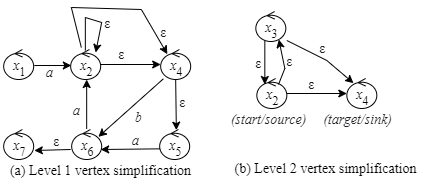
\includegraphics[]{../figures/vertexSimplification.png}
    \caption{The levels 1 and 2 vertex simplification $R_1$ and $R_2$ of the RLDT in \ref{sampleRDLT} (Image Source: \cite{MalinaoWCTP2023})}
    \label{vertexSimplification}
\end{figure}
% -------------------------------------------
\subsection*{$L$-Safeness of RDLTs}
% include here the defintions from kuya Ronnie's
% add paragraph introducing L-safeness of RDLT
In the analysis of processes in RDLT, particularly on its verification of soundness property, it is crucial that possible $L$-attrbute-based deadlocks are avoided. Reachability of the vertices relies heavily on the configuration of the arcs' $L$-values, along with other factors such as connectivity, and $C$-attributes. The following definitions discusses the $L$-safeness with RDLTs from \cite{MalinaoPJS2023}.
\begin{defn}\textbf{Critical and Escape Arcs} \cite{MalinaoPJS2023}
    A cycle $ c $ $ = $ $ [ x_1 x_2 \ldots x_n ] $ is a sequence of vertices $ x_i $ $ \in $ $ V $, where $ (x_i,x_{i+1}) $ $ \in $ $ E $, $ i $ $ = $ $ 1,2, \ldots, n - 1 $, and no two vertices in $ c $ are the same except for $ x_1 $ $ = $ $ x_n $. The elements of $ c $ are denoted as $ Lit(c) $. We denote the set of arcs of $ c $ as $ ArcsOfCycle(c) $ $ = $ $ \{ (x,y) $ $ \in $ $ E | \exists x_i, x_{i+1} $ $ \in $ $ Lit(c) $ where $ x $ $ =  $ $ x_i $ and $ y $ $ = $ $ x_{i+1} \} $.

    $ (x,y) $ $ \in $ $ ArcsOfCycle(c) $ is called a critical arc (CA) in $ c $ if it has the minimum $ L $-value among the arcs in $ c $, i.e. $ L(x,y) $ $ = $ $ min_{(u,v) \in ArcsOfCycle(c) } \{L(u,v)\} $. If $ \exists (x,v) $ $ \in $ $ E $ such that $ v $ $ \in $ $ V \backslash Lit(c) $, then we refer to $ (x,v) $ as an escape arc (EA) of $ (x,y) $ in $ c $. Self-loops, i.e. $ (x,x) $, are cycles that are themselves entirely composed of one critical arc that does not affect the (re)use of other arcs in an RDLT.
\end{defn}

An example of a \textbf{cycle} is $x_2$, $x_3$, where the arc from $x_3$ eventually leads to $x_2$, where $x_3$ can be traced, as well. The \textbf{critical arc} in this cycle is the arc with the minimum $L$-attribute, which is $(x_2, x_3)$. Hence, the rest of the arcs in this cycle is a \textbf{non-critical arc}, e.g., the arc $(x_3,xx_2)$. The \textbf{escape arc} will be the arc $(x_2,x_4)$.

\begin{defn}\textbf{Loop-Safe Arcs} \cite{MalinaoPJS2023}
    \label{LSA}
    Let $ R $ be a connected RDLT, i.e. for every vertex $ v $ $ \in $ $ V $, there is a path from a source vertex $ s $ $ \in $ $ V $ to $ v $ in $ R $. A non-critical arc (NCA) $ (x,y) $ $ \in $ $ E $ of $ R $ is loop-safe if $ L(x,y) $ $ > $ $ RU(x,y) $, where
    \begin{gather*}
        RU(x,y) = \Sigma_{k=1^{|Cycles(x,y)|}} (I * L(u,v)) \text{, for some } (u,v) \in minL\_CA(c_k) \text{, with} \\
        I =
        \begin{cases}
            1, & \text{if } k = 1 \text{ or } \cup_{j=1^{k-1}} minL\_CA(c_j) \cap minL\_CA(c_k) \\
            0, & \text{otherwise,}
        \end{cases}
    \end{gather*}
    and $ minL\_CA(c) $ $ \subset $ $ E $ is the set of arcs whose $L$-value is the minimum among the critical arcs found in $ c $, accounting the other cycles in $ c' $ in $ R $ that intersect with $ c $.
\end{defn}

\begin{defn}\textbf{Safe Critical Arcs} \cite{MalinaoPJS2023}
    \label{SafeCA}
    A CA $ (x,y) $ $\ in $ $ E $ is safe if there is an escape, non-critical arc $ (x,z) $ $\ in $ $ E $, where $ (x,z) $ is loop-safe.
\end{defn}

In general, escape arcs ensure that the workflow can escape from a cycle whenever the critical arc is fully used in an activity. However, having a safe critical arcs and loop-safe NCAs in $R$ is insufficient in achieving complete soundess. In ensuring $R$ is classically sound, an added requirement,that of $JOIN$-safe $L$-values, on an $R$ having no $RBS$.

\subsubsection*{JOINs in RDLTs}
In RDLTs, it is not impossible for multiple processes to converge at a single vertex (JOIN). The type of join specifies how the incoming processes interact before proceeding in the workflow. The following definitions are the different types of joins in RDLTs:
\begin{itemize}
    \item[1.] AND-JOIN at $y \in V$: For every type-alike arcs $(v,y), (u,y) \in E$ where $(v,y) \neq (u,y)$, their C-values $C(v,y) \neq C(u,y)$ and $C(v,y),C(u,y) \in \Sigma$.
    \item[2.] MIX-JOIN at $y \in V$: There is at least one pair of type-alike arcs $(v,y), (u,y) \in E$ where $(v,y) \neq (u,y)$, $C(v,y) \neq C(u,y)$ and $C(v,y) = \epsilon$, and $C(u,y) \in \Sigma$.
    \item[3.] OR-JOIN: For every type-alike arcs $(v,y), (u,y) \in E$ where $C(v,y)=C(u,y)$.
\end{itemize}

The concept of JOIN-safe $L$-values aids in ensuring the $JOIN$-safeness of an RDLT. This is one of the helpful design strategies to achieve classical soundness in JOINs, as discussed the paper \cite{MalinaoPJS2023}. This, along with defintions \ref{LSA} and \ref{SafeCA}, provides the structural requirement for a classically sound RDLT, e.g, proper termination and liveness. These definitions serves as the basis for determining looser notions of soundness.

\begin{defn}\textbf{JOIN-safe $L$-values} \cite{MalinaoPJS2023}
    \label{JSL}
    For every pair of arcs $(u, y)$, $(v, y)$ $ \in $ $ E $, where $C(u, y)$ $ \neq $ $C(v, y)$, we say that $(u, y)$ and $(v, y)$ have JOIN-safe $L$-values if:

    \begin{enumerate}
        \item \textbf{One split origin.} There is exactly one common ancestor $ x $ $ \in $ $ V $ for $ u $ and $ v $ such that there is exactly one path $ P_u $ $ = $ $ a_1 a_2 \ldots a_n $, where $ a_1 $ $ = $ $ x $, $ a_{n-1} $ $ = $ $ u $, $ a_n $ $ = $ $ y $, $ a_i $ $ \in $ $ V $, $ 1 < I < n - 2 $, and another path $ P_v $ $ = $ $ b_1 b_2 \ldots b_m $, where $ b_1 $ $ = $ $ x $, $ b_{m-1} $ $ = $ $ v $, $ b_m $ $ = $ $ y $, $ b_j $ $ \in $ $ V $, $ 1 < j < m - 2 $. Furthermore, $ P_u $ and $ P_v $ do not intersect with each other except at $ x $ and $ y $. That is, no $ a_i $ and $ b_j $ along these paths are equal, for $ 1 < i < n $ $ 1 < j < m $; and
        \item \textbf{No unrelated process.} For every arc $ (a,b) $ $ \in $ $ E $, if $ a $ $ = $ $ x $, where $x$ is the one common ancestor of $u$ and $v$, then there is no path from $a$ to another vertex $r$ $\in$ $V$ such that for some $(r,s)$ $\in$ $ E $, $s$ $\neq$ $y$.
        \item \textbf{No branching out from every related process.} $\forall q_k $ $ \in $ $ Lit(P_q) $, where $ q $ $ \in $ $ \{u,v\} $, $ 1 \leq k < |Lit(P_q)| $, $ \nexists (q_{k,s}) $ $ \in $ $ E $ where $ s $ $ \in $ $ V \backslash Lit(P_q) $.
        \item \textbf{No process interruptions.} $ \forall q_k $ $ \in $ $ Lit(P_q) $, where $ q $ $ \in $ $ \{u,v\} $, $ 1 < k \leq |Lit(P_q)| $, $ \nexists (s,q_{k}) $ $ \in $ $ E $ where $ s $ $ \in $ $ V \backslash Lit(P_q) $.
        \item \textbf{Duplicate conditions.}
        \begin{itemize}
            \item If $ C(u,y) $, $ C(v,y) $ $ \in $ $ \Sigma $, i.e. an AND-JOIN at $ y $, then there is no process $ P $ $ = $ $ [x_1 x_2 \ldots x_p] $ in $ R $, where $ x_1 $ $ = $ $ x $, $ x_p $ $ = $ $ y $, such that $ C(x_{p-1}, x_p ) $ $ = $ $ C(u,y) $ (or $ C(v,y) $).
            \item Without any loss of generality, if $ C(u,y) $ $ = $ $ \varepsilon $ and $ C(v,y) $ $ \in $ $ \Sigma $, then any process $ P $ $ = $ $ x_1 x_2 \ldots x_p $ in $ R $, where $ x_1 $ $ = $ $ x $, $ x_p $ $ = $ $ y $, can have $ C(x_{p-1}, x_p) $ $ \in $ $ \{\varepsilon, C(v,y)\}$. That is, a MIX-JOIN can have duplicate conditions for the arcs connecting to $y$, but no two of such arcs have different conditions.
        \end{itemize}
        \item \textbf{Equal $ L $-values of arcs at the AND-JOIN.}
        \item \textbf{Loop-safe components of every related process.} For an AND- or MIX-JOIN merging at $y$, each of its processes $ P $ $ = $ $ x_1 x_2 \ldots x_k $, $ k $ $ \in $ $ \mathbb{N} $, where $ x_1 $ $ = $ $ x $ and $ x_k $ $ = $ $ y $, the arc $ (x_1, x_{i+1}) $ $ \in $ $ E $. $ i $ $ = $ $ 1, 2, \ldots, k - 1 $, is loop-safe. Lastly, for an OR-JOIN merging at $ y $, each process $ P $ $ = $ $ x_1 x_2 \ldots x_k $, $ k $ $ \in $ $ \mathbb{N} $, of this JOIN has its arc $ (x_i,x_{i+1}) $ to have a JOIN-safe L-value, $ i $ $ = $ $ 1, 2, \ldots, k - 1 $, if $ (x_i, x_{i+1}) $ is either a loop-safe arc or a safe CA in R.
    \end{enumerate}
    
\end{defn}
% -------------------------------------------
\subsection*{Reusability and Resets in RDLTs}
The concept of reusability refers to how components of an RDLT can be used in different situations, such as when an RDLT has at least one RBS \cite{MalinaoWCTP2023}. The information in this section is sourced from \cite{MalinaoWCTP2023} unless explicitly mentioned otherwise.


\begin{defn} Pseudocritical Arcs, Pseudo-escape Arcs \\
A pseudocritical arc $(PCA) (x,y) \in E$, where $(x,y)$ is a component of a cycle $c$ in $R$ where $L(x,y$) is the minimum among all the L-values of the arcs in $c$ which are not arcs of an RBS in $R$.

Meanwhile, a pseudo-escape arc $(PEA) (x,z) \in E$ is a non-critical arc in $R$ where $(x,y)$ and $(x,z)$ are type-alike.    
\end{defn}

\begin{defn} Expanded Reusability in RDLTs with Resets \\
Let $R =  (V, E, T, M)$ be a connected $RDLT$. If $\exists v \in V$ where $M(v)=1$, then let $B =  (V', E', T', M')$ be the RBS with its center $v$.
\begin{enumerate}
    \item Let $IB_r(X)$ be the set of in-bridges of $x \in V$.
    \item Let $Cycles_{part}(R)$ be a set of cycles in $R$ with the following property: $\forall p = [x_1 x_2 ... x_n] \in Cycles_{part}(R)$, there exist cycle components meeting these conditions:
    \begin{itemize}
        \item [(a)] $(x_i,x_{i+1}) \in E$ is inside an RBS $B$ of $R$ (i.e, $x_i,x_{i+1} \in V'$).
        \item [(b)] $(x_j,x_{j+1}) \in E$ is not inside $B$ (i.e, $x_j or x_{j+1} is not in V'$).
    \end{itemize}
\end{enumerate}
Whenever we have cycles $d = [d_1 d_2 ... d_{m1}], e = [e_1 e_2 ... e_{m1}] \in Cycles_{part}(R)$ that overlap in their non-RBS components, and this overlap contains both of their PCAs $(d_k,d_{k+1}), (e_{k'},e_{k'+1})$, where $L(d_k,d_{k+1}) \geq L(e_{k'},e_{k'+1})$, then consider only one of these PCAs. Choose the one with the minimum L-value as it would ultimately contribute to the reusability of every RBS component reachable from these cycle components.
\end{defn}

\begin{defn} (RU-preserving transformation) \\
    A transformation $\delta$ of an input RDLT $R$ to another RDLT $R'$ is said to be RU-preserving if for every activity profile $S = {S(1), S(2), ..., S(n_1)}, n_1 \in IN$, that is derivable from $R$, there is a corresponding activity profile $S' = {S'(1), S'(2), ..., S'(n_2)}, n_2 \in IN$, that is derivable from $R'$, where for every pair $(x,y) \in S(i)$ and $(y,z) \in S(i+1)$, either of the following holds:
    \begin{enumerate}
        \item $(x,y) \in S'(j)$ and $(y,z) \in S'(j+1)$,
        \item there exists a path $p=x_1, x_2, ..., x_n \in R$ being represented by the arc $(x_1, x_n)$ in $R$ being represented by the arc $(x_1, x_n)$ in $R'$ where $x_{k-1}=x,x_k, x_{k+1}=z$, and
            \begin{itemize}
                \item[(a)] $(s,x_1) \in S'(j)$ and $(x_1,x_n) \in S'(j+1)$, for some vertex $s$ in $R'$,
                \item[(b)] $(x_1,x_n) \in S'(j)$, for some $1 \leq j \leq n_2$, or
                \item[(c)] $(x_1,x_n) \in S'(j)$ and $x_n$, $s \in S_{j-1}$, for some vertex $s$ in $R'$.
            \end{itemize}
    \end{enumerate}
    Furthermore, we call $(x_1,x_n)$ as the abstract arc in $R'$ representing the path $p$ in $R$.
\end{defn}
% -------------------------------------------
\subsection*{Expanded Vertex Simplification}
The process of vertex simplification results to an RDLT $R$ lacking of $L$-values. Therefore, \cite{MalinaoWCTP2023} proposes and extension of the process to produce \emph{expanded vertex simplifiction} $R_1'$ and $R_2'$ with respect to $R$ by using the RDLT and its simplified vertex to retrieve the other attributes, e.g. $L$. The algorithm for producing $R_1'$ and $R_2'$ is outlined in algorithm \ref{EVSA}, found in the appendices.

\begin{figure}[H]
    \centering
    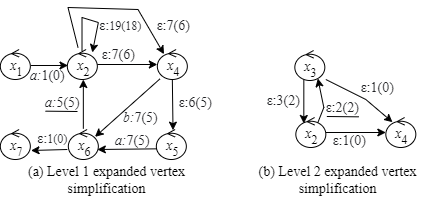
\includegraphics{../figures/expandedVertexSimplification.png}
    \caption{$R_1'$ and $R_2'$ expanded vertex simplification of the vertex simplified graphs in Figure \ref{vertexSimplification}}
    \label{expandedVertexSimplifiedRLDTs}
\end{figure}


% -------------------------------------------
\subsection*{Soundness Property in RDLT}
As explained in earlier sections, the existence of formalizations on the notions of soundness in Workflow nets served as the foundation for the formalizations of soundness on RDLT. Included in the list are classical and relaxed soundness, as formalized by \cite{Malinao2017}, and weak and easy soundness by \cite{Ramirez2024}, all in the context of notions of soundness. The first two notions of soundness are defined below.
\begin{defn}\textbf{Classical Soundness of RDLTs} \cite{MalinaoPJS2023}
    \label{ClassicalRDLTDef}
    An RDLT is of classical sound if and only if the following requirement is satisfied by each activity profile $ S = \{S(1), S(2), ..., S(k)\}, 1 \leq k \leq diam(R), diam(R) $ is the diameter of $ R $, of a set of source vertices $ I $ $ \subset $ $ V $ and a final output vertex $ f $ $ \in $ $ V, $ where $ \forall $ $ x $ $ \in $ $ I $ and $ y $ $ \in $ $ V $, $ (x,y) $ $ \in $ $ S(1), $ and $ (u,f) $ $ \in $ $ S(k) $, $ u $ $ \in $ $ V $:
    \begin{enumerate}
        \item \textbf{Proper termination.} For every activity profile $ S = \{S(1), S(2), ..., S(k)\}, 1 \leq k \leq diam(R) $, of a set of source vertices $ I $ $ \subset $ $ V $ and a final output vertex $ f $ $ \in $ $ V $.
        \begin{itemize}
            \item All arcs in the final reachability configuration $ S(k) $ must be incident to sink $ f $, i.e. for every $ (x,y) $ $ \in $ $ S(k), $ $ y = f $
            \item If $ k $ $ \leq $ $ 2 $: every arc incident to a vertex $ y $ in a reachability configuration $ S[i] $ has a corresponding arc incident from vertex $ y $ in a succeeding reachability configuration $ S(j) $, $ i.e. $ for every $ (x,y) $ $ \in $ $ S[i] $, there exists another arc $ (y,z) $ $ \in $ $ S(j) $, for all $ 1 \leq i < k $, and for some $ j $ in the range $ i + 1 \leq j \leq k $.
        \end{itemize}
        \item \textbf{Liveness.} Every arc is traversed in some activity profile, $ i.e. $ for every $ (x,y) $ $ \in $ $ E $, there is an activity profile $ S' = \{S'(1), S'(2), ..., S'(k')\} $, where $ (x,y) $ $ \in $ $ S'[i], 1 \leq k \leq k' $.
    \end{enumerate}
\end{defn}

Based on this definition, the first condition requires an RDLT \emph{R}'s each specified vertex and their subsequent vertices leading to the final vertex of \emph{R}. All required component of a JOIN is already resolved, or checked, by the activity extraction algorithm upon termination. In other words, an RDLT needs to have proper termination for each of its activity profiles. The second condition requires it to have no possible occurences of deadlocks for every component in the RDLT as it requires that all arcs are to be included in an activity profile during extraction, i.e., liveness of the RDLT. Figure \ref{sampleRDLT} satisfies both conditions an is therefore classically sound.

\begin{defn}\textbf{Relaxed Soundness of RDLTs} \cite{Malinao2017, MalinaoPJS2023, Sulla2023}
    \label{RelaxedRDLTDef}
    An RDLT is of relaxed sound if for every sink $ f $ $ \in $ $ V $ and a source $ w $ $ \in $ $ R $, where $ w $ is an ancestor of $ f $, there exists an activity profile $ S = {S(1), S(2), ..., S(k)} $, where $ 1 \leq k \leq diam(R) $, where the following conditions hold:
    \begin{itemize}
        \item For every reachability configuration $ S(t) $ prior to $ S(k) $, if any, there should be at least one arc $ (x,y) $ $ \in $ $ S(t) $ and another arc $ (y,z) $ $ \in $ $ S(t') $, for a time $ t' $, where $ t < t' \leq k $. This ensures that there is at least one continuous path from $ w $ to $ f $ in activity $ S $.
        \item The final reachability configuration $ S(k) $ is only composed of arcs that point to the sink $ f $, $ i.e. $ $ \forall (x,y) $ $ \in $ $ S(k) $, $ y = f $.
        \item The set of arcs traversed at a time $ t $ is strictly contained in the set of arcs traversed at time $ t + 1 $, $ i.e. $ $ \bigcup_{i=1}^{t} S[i] $ $ \subset $ $ \bigcup_{i=1}^{t+1} S[i] $. Since an arc can occur in multiple $ S[i] $, the operator $ \bigcup $ should be considered a multiset union operator.
        \item Every arc $ (x,y) $ $ \in $ $ E $ is traversed in some activity profile $ S' $, $ i.e. $ there exists an activity profile $ S' $, where $ (x,y) $ $ \in $ $ S'(t) $ for some $ S'(t) $ $ \in $ $ S' $.
    \end{itemize}
\end{defn}

% Relaxed soundness refers to a notion of soundness with a weakened property that of proper termination. At least only one vertex is required to be leading to the final vertex, in contrast to a classically sound RDLT. This is given by the first, third, and fourth requirement. The liveness, however, is retained as defined in the second and third requirement, preventing deadlocks. Meaning, a relaxed soundness is live.  The RDLT therefore in Figure \ref{sampleRDLT} is relaxed sound, aside from the fact that it is classically sound in the first place. - Feedback 4.14.d (RESOLVED)

In summary, relaxed soundness in the context of RDLT, follows the notion of relaxed soundness to that of a Workflow Net PN. It follows that the condition of proper termination of a classically sound RDLT is relaxed or weakened, that is, for an RDLT to be of relaxed soundness it is only required that there be at least one activity profile where proper termination is obeserved, while still retaining the condition of liveness of a classically sound RDLT.
% State Representation
% Activity Extraction 

% -------------------------------------------


\section{Problem Statement}
\label{sec:ProbStmnt}
% Matrix representation is used to extract activities from an RDLT, using computations involving matrix operations. The purpose of this research is to verify the weak and easy soundness of an input RDLT using these operations. Karen and Roben \cite{KarenRoben2018} and Asoy \cite{Asoy2024} already conducted studies involving the matrix representation of relaxed and classical soundness, respectively. Similarly, the recently formalized notion of soundness, that of weak and easy soundness in RDLT \cite{Ramirez2024}, provided a behavioral and structural profile upon which algorithms were proposed for the verification thereof. The problem statement of this paper is to create a matrix representation for the verification of weak and easy soundness of RDLT, based on its formalizations. TODO: To be revised as in Feedback 5.1

The verification of soundness properties of RDLT can be done through the analysis of its L-safenesss, as done in \cite{MalinaoPJS2023}. Matrices can then be used, as done in the papers \cite{KarenRoben2018} and \cite{Asoy2024}, to represent the RDLT information, e.g. the vertices and arcs, the attributes, the check/traversal components, and the entire state of the RDLT during execution up until execution. The matrix representation of an RDLT is then used for the verification of classical soundness and relaxed soundness in papers \cite{Asoy2024} and \cite{KarenRoben2018}, respectively. In the context of this study, the notions of weak and easy soundness of RDLT was just recently formalized, along with the verification strategy, in the paper of \cite{Ramirez2024}. This study is therefore centered on the matrix representation, and using related operations, to verify weak and easy soundness of RDLT, along with the creation of matrix-based data structures, relying on the methods and formalizations of the aforementioned studies. The lack of a well-defined matrix representation tailored to the verification of weak and easy soundness of RDLT, based on recent formalizations, presents a gap in the literature that this study aims to address.

% Due to the importance of the verifying weak and easy soundness of a system, the use of matrix representation and operation in the verification thereof could lead to an improved method for the automation of verifying systems. This deepends the theoretical framework of RDLT and strengthens its applica in systems design. By establishing this method, we address gaps and contribute to te boarder understanding of the field by:


% objectives of the study
\section{Aim of the Work}
\subsection*{General Objectives}
Currently, there are already existing literature on weak and easy soundness in the context of RDLT. However, in the case of this research, the matrix representation for the verification of these notions of soundness is to be addressed. Therefore, the general objective of the study is the following:

\begin{enumerate}
    \item To design a matrix based representation of RDLT, and related matrix operations, for the verification of weak and easy soundness; as well as to implement the verification algorithm of \cite{Ramirez2024} for the verification of weak and easy soundness using matrix representation.
\end{enumerate}

\subsection*{Specific Objectives}
In alignment with the general objectives, the following specific objectives are identified to reach these aims:
\subsubsection*{For Weak Soundness Structural Verification}
\begin{enumerate}
    \item To establish matrix representation and operations for the verification of deadlock tolerance in both level 1 and level 2 expanded vertex simplification graphs \cite{MalinaoWCTP2023}, $R_1$ and $R_2$, respectively, of RDLT $R$ \cite{Malinao2017}.
    \item To generate a list of deadlock points in $R$ and identify escape contraction paths \cite{Ramirez2024} \cite{MalinaoPJS2023}.
    \item To establish matrix representation and operations to verify weakened join-safe values of every split-join \cite{Ramirez2024} pair in $R$.
    \item To establish matrix representation and operations for the verification of weakened-join safeness \cite{Ramirez2024} of $R$.
    \item To verify the loop-safeness of NCA and safeness of CA \cite{MalinaoPJS2023}.
    \item To establish matrix representation and operations for the verification that $R$ is deadlock-resolving \cite{Ramirez2024}.
    \item To formulate test cases to prove the correctness of the proposed matrix represention and operations in verifying weak soundness of RDLTs \cite{Ramirez2024}.
    \item To prove the correctness of the proposed matrix representation and operations in verifying weak soundness of RDLTs \cite{Ramirez2024}.
    \item To measure the time and space complexity of the matrix-based verification of weak soundness of $R$.
\end{enumerate}
\subsubsection*{For Easy Soundness Structural Verification}
\begin{enumerate}
    \item To formulate test cases to prove the correctness of the proposed matrix represention and operations in verifying easy soundness of RDLTs \cite{Ramirez2024}.
    \item To prove the correctness of the proposed matrix representation and operations in verifying easy soundness of RDLTs \cite{Ramirez2024}.
    \item To measure the time and space complexity of the matrix-based verification of easy soundness of R.
\end{enumerate}
% scopes and limitations
\section{Scope and Limitations}
The scope and limitations of the study are the following:
\begin{enumerate}
    \item The study will focus on the design of matrix representation that encapsulates the structure of RDLT. It will incorporate matrix operations on the verification of the structural profiles of RDLT, as discussed in the paper of \cite{Ramirez2024} to determine its weak and easy soundness. The study will not delve to alternative models other than matrix representation.
    \item The study will center on RDLT as the main structural model to verify notions of soundness with \cite{Malinao2017}. Furthermore, its level 1 and level 2 expanded vertex simplified graphs will be used in the verification of weak soundness \cite{MalinaoWCTP2023}. The study will not explore other types of models beyond these graphs.
    \item The study will center on the verification of weak and easy notions of soundness \cite{Malinao2017} \cite{Ramirez2024}. Its structural profiles will be used for the verification. The study does not include other notions of soundness.
    \item The study will focus on verifying deadlock tolerance in the context of RDLT, as defined in the structural profile of weak soundness \cite{Ramirez2024}. The study is limited to the definition of deadlock tolerance within this context.
    \item The study aims to design and implement a matrix-based verification algorithms for weak and easy notions of soundness of an RDLT. The algorithms are only limited to weak and easy soundness and will not perform matrix operations beyond these verifications.
\end{enumerate}

% significance of the study
\section{Significance of the Study}
\indent The study and its results will contribute to the enhanced understanding of RDLT and the verification of notions of soundness. Specifically, the study is centered on the matrix-representation of RDLT to verify weak and easy soundness, which could lead to improved methods for the analysis and modeling of complex systems. This deepens the theoretical framework of RDLT and strengthens its applicability in systems design. By establishing matrix-representation and operations for the verification of these notions of soundness, we address gaps and contirbute to the broader understanding of the field by:
\begin{enumerate}
    \item Providing a structured framework for the verification of easy and weak soundness, which could lead to the enhancement of reliablity and accuracy of complex systems.
    \item Introduce efficient deadlock detection and resolution mechanisms through matrix-based operations, leading to more robust systems.
    \item Providing the groundwork for the advancement of automated verification tools, speeding up the validation process of RDLTs, in the scope of weak and easy notions of soundness.
\end{enumerate}

\section{Theoretical and Conceptual Framework}
\label{sec:TCF}
The Figure presents the conceptual framework of the research. It contains required concepts and definitions in order to proceed with the methodology and achieve the reseach objectives. 

The main requirements for achieving the main objectives of the research are the following: definition of RDLT \cite{Malinao2017}, definition of a weak and easy sound RDLT based on their structural and behavioral profiles \cite{Ramirez2024}, RDLT Activity extraction \cite{Malinao2017} \cite{Asoy2024}, Vertex Simplification, and Matrix Operations \cite{KarenRoben2018}. RDLT is defined in \cite{Malinao2017} and the classical notion of soundness. By the scope of this research, the weak and easy notions of soundness are to be verified, the profiles and algorithm of which are already defined by \cite{Ramirez2024}. Majority of the research's objectives is focused on the matrix-based verification of the deadlock tolerance (and its subsequent properties) of the input RDLT \cite{Ramirez2024}. This methodology requires expanded vertex simplification \cite{MalinaoWCTP2023} (both level-1 and level-2) and a proposed algorithm for activity extraction \cite{Malinao2017}. Finally, the final state vector output of the matrix operations on the input RDLT will be evaluated for its validity, then its weak and easy soundness.

The implementation of this research would therefore include the reusing of the definitions of RDLT \cite{Malinao2017}, weak and easy soundness profiles \cite{Ramirez2024}, and the algorithm for the verification thereof. The algorithm by \cite{Ramirez2024} would be translated or modified to verify a matrix-based RDLT. To achieve these main objectives, specific objectives are to be achieved first, requiring the same set of concepts and algorithms. Finally, after formulating the test cases for verifying the correctness of the matrix-based verification of weak and easy soundness, the time and space complexity will also be performed. 

Below is the concpetual framework Figure \ref{conceptualFramework} which shows the concepts and components from related literature that are required to implement the objectives, displayed as yellow boxes, as well as the components for the implementations to satisfy the objectives of this study. This includes modified and novel methods, shown by orange and green boxes, respectively.

% \newgeometry{landscape, width=1\textwidth, height=\textheight, left=1in, right=1in, top=3in, bottom=1in}
% \begin{landscape}
%     \begin{figure}[htbp]
%         \label{conceptualFramework}
%         \centering
%         \includegraphics[width=1.6\textwidth]{figures/TCF.png}
%         \caption{This framework shows the requirements of the research's framework, with its main components, namely: Matrix Representation, Behavioral and Structural Profile of the RDLT.}
%     \end{figure}
% \newpage
% \end{landscape}
% \restoregeometry

% \newpage
% \begin{figure}[htbp]
%     \centering
%     \includegraphics[width=1\textheight]{../Figures/TCF.png}
%     \caption{A beautiful image.}
%     \label{fig:nature}
% \end{figure}
 
\newpage
% \begin{landscape}
%     \begin{figure}[htbp]
%         \section{Schedule of Activities}
%         \centering
%         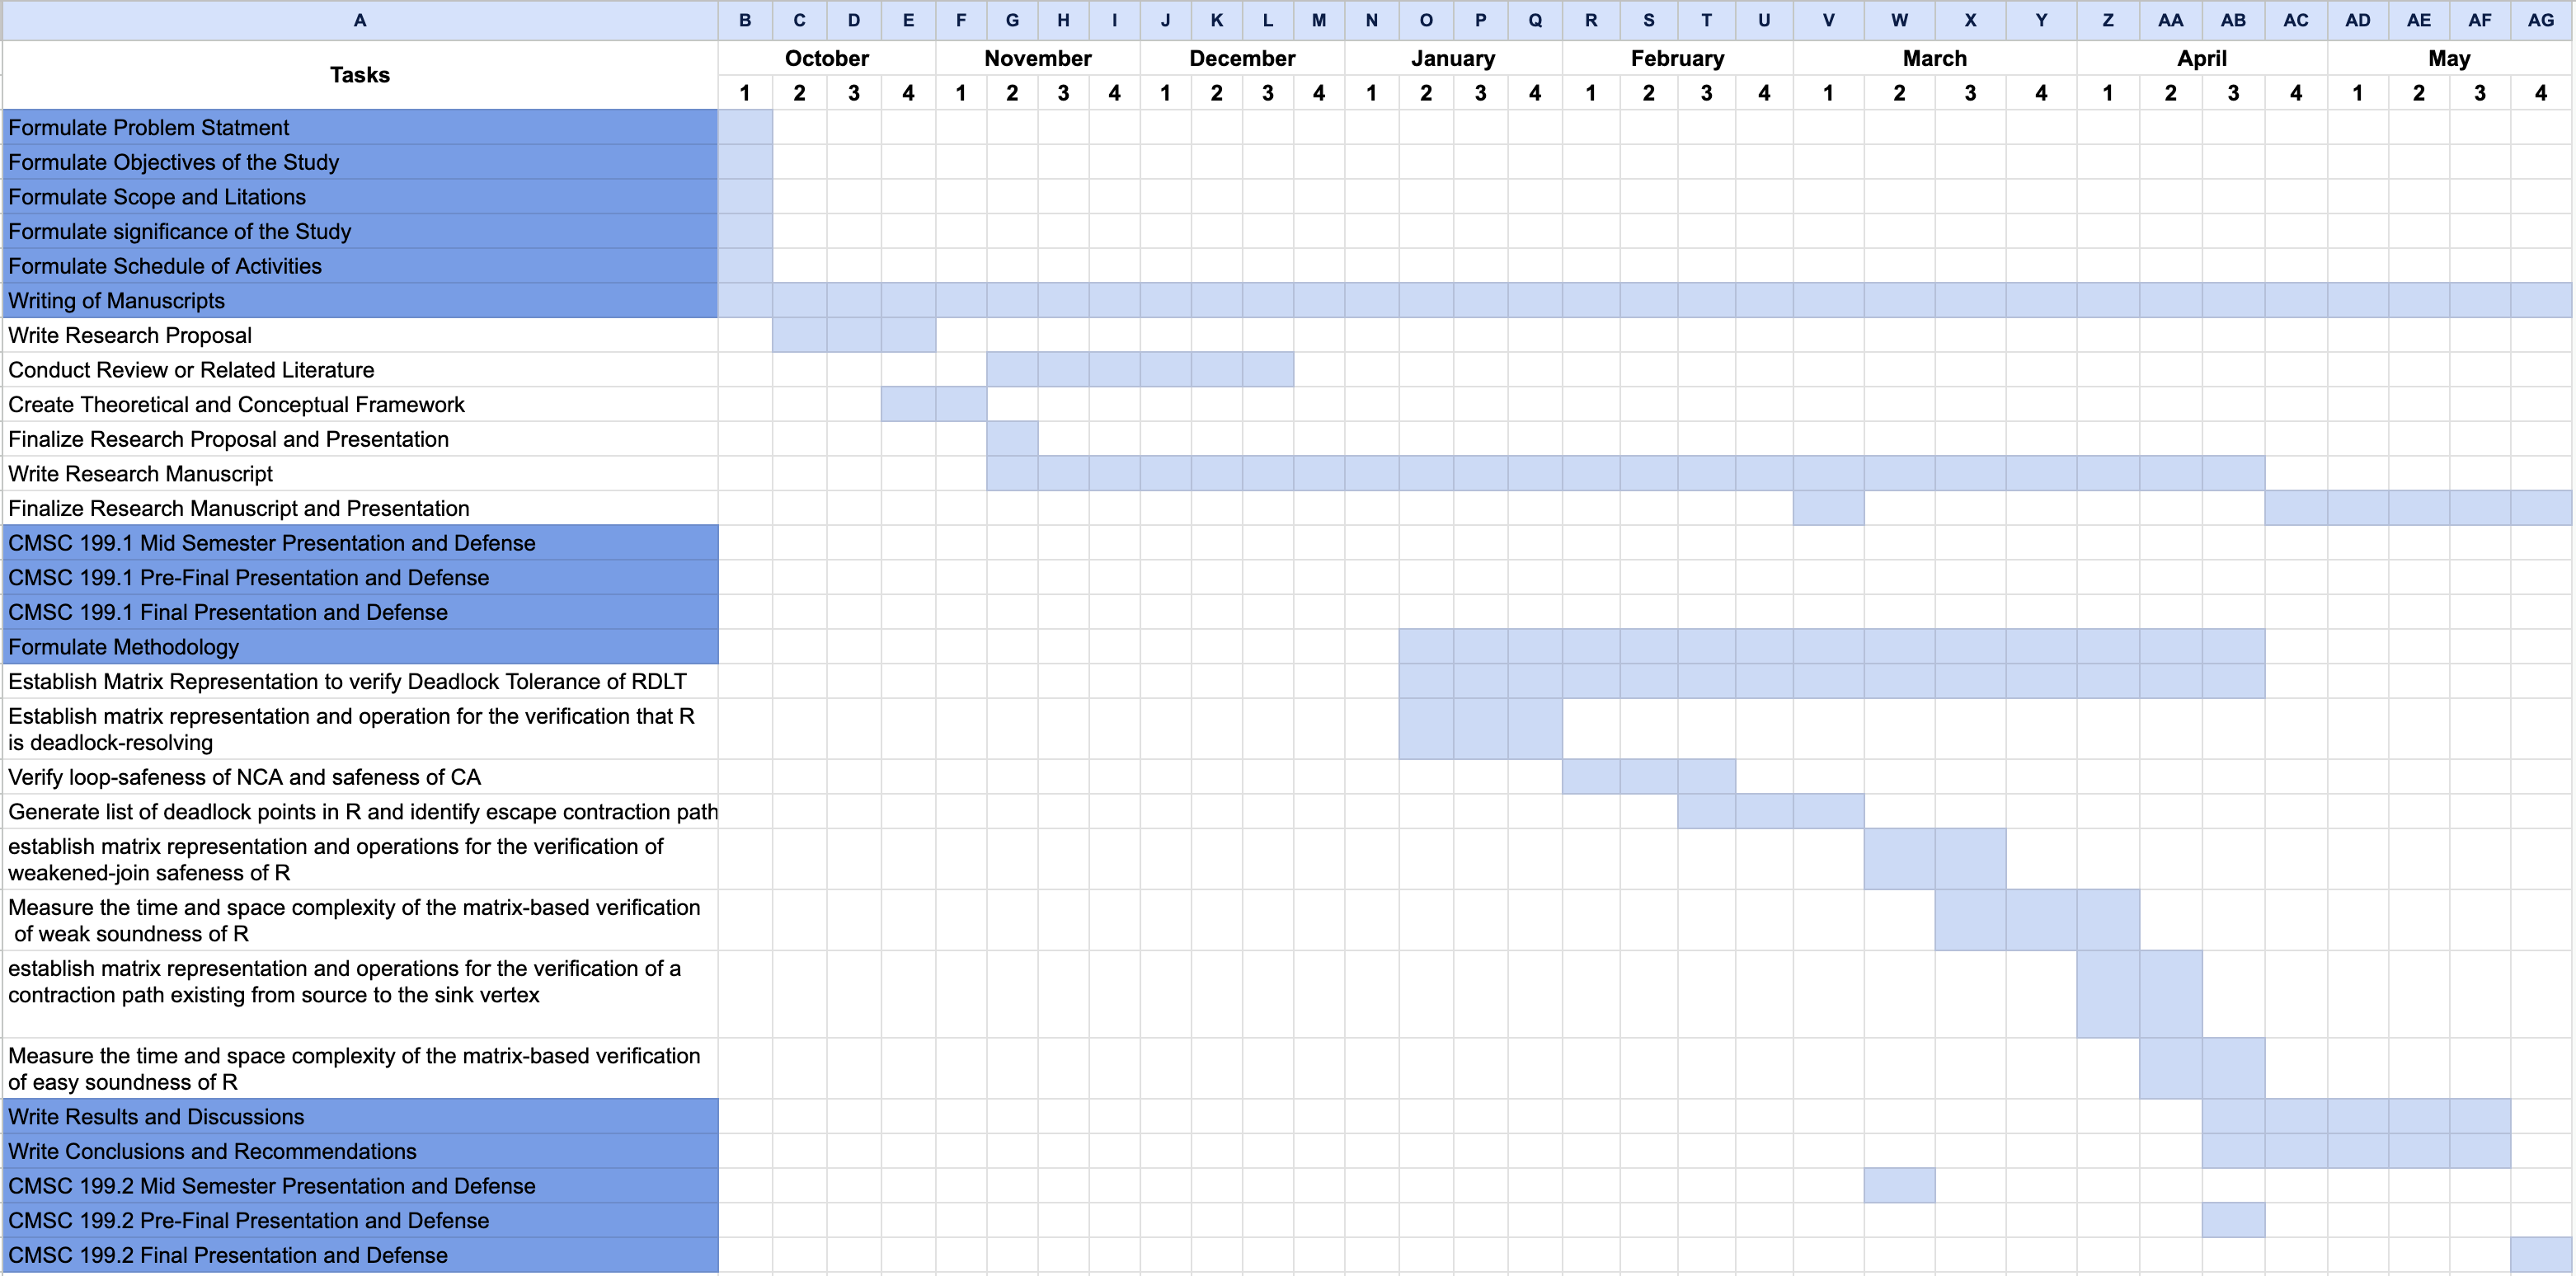
\includegraphics[width=1.5\textwidth]{figures/sched.png}
%         \caption{Proposed Schedule for the Implementation of the Research Activities}
%     \end{figure}
% \end{landscape}


